%%%%%%%%%%%%%%%%%%%%%%%%%%%%%%%%%%%%%%%%%%%%%%%%%%%%%%%%%%%%%%%
%
% Welcome to Overleaf --- just edit your LaTeX on the left,
% and we'll compile it for you on the right. If you open the
% 'Share' menu, you can invite other users to edit at the same
% time. See www.overleaf.com/learn for more info. Enjoy!
%
%%%%%%%%%%%%%%%%%%%%%%%%%%%%%%%%%%%%%%%%%%%%%%%%%%%%%%%%%%%%%%%


% Inbuilt themes in beamer
\documentclass{beamer}

% Theme choice:
\usetheme{CambridgeUS}
\usepackage{amsmath}

\usepackage{array}
\newcolumntype{P}[1]{>{\centering\arraybackslash}p{#1}}

% Title page details: 
\title{AI1110: Probability and Random Variables}
\subtitle{Assignment 7: Papoulis-Pillai Ex 4-22}
\author{Rishit D (cs21btech11053)}
\institute{IIT Hyderabad}
\date{\today}


\begin{document}

% Title page frame
\begin{frame}
    \titlepage 
\end{frame}

% Outline frame
\begin{frame}{Outline}
    \tableofcontents
\end{frame}

% Problem
\section{Problem}

\begin{frame}{Assignment 6}
  \frametitle{Problem}
  The probability of \emph{heads} of a random coin is a random variable $p$ uniform in the interval (0.4,0.6).
  \begin{enumerate}
  \item Find the probability that at the next tossing of the coin \emph{heads} will show.
  \item The coin is tossed 100 times and \emph{heads} shows 60 times. Find the probability that at the
next tossing \emph{heads} will show.
  \end{enumerate}
\end{frame}

% Solution
\section{Solution}
\subsection{Part 1}

%Defining PDF (1st idea)
\begin{frame}
  \frametitle{Defining PDF}
  We will define the probability density function $f(p)$ as follows 
  \begin{align}
    f(p) = 
    \begin{cases}
      5, & p \in (0.4, 0.6) \\
      0, & \text{otherwise}
    \end{cases}
    \label{eq:Dis1}
  \end{align}

  Note that we ensure that the area under the probability density function $f(p)$ is 1.
\end{frame}

%Finding probability of getting head
\begin{frame}
  \frametitle{Finding probability of getting Heads}
  The total probability theorem in continuous form states
  \begin{block}{Total Probability Theorem}
    \begin{align}
      \Pr(A) = \int_{-\infty}^{\infty}\Pr(A|p)f(p)dp
      \label{eq:TotProb}
    \end{align}
  \end{block}

  Using
  \eqref{eq:TotProb}
  we have
  \begin{align}
    \Pr(H) = \int_{-\infty}^{\infty} \Pr(H|p)f(p) dp
    \label{eq:InitialHead1}
  \end{align}
  
\end{frame}

\begin{frame}
  \frametitle{Finding probability of getting Heads}

  Using
  \eqref{eq:Dis1}
  in
  \eqref{eq:InitialHead1}
  \begin{align}
    \Pr(H) = \int_{0.4}^{0.6} 5\Pr(H|p) dp
    \label{eq:InitialHead2}
  \end{align}

  Note that we define the random variable p such that it represents the probability that a coin toss results in a \emph{Head}. Hence
  \begin{align}
    \Pr(H|p) = p
    \label{eq:ProbRV}
  \end{align}

  Using
  \eqref{eq:ProbRV}
  in
  \eqref{eq:InitialHead2}
  \begin{align}
    \Pr(H) = \int_{0.4}^{0.6} 5p dp = \fbox{0.5}
    \label{eq:InitialHeadProb}
  \end{align}
    
\end{frame}

\begin{frame}
  \frametitle{Code Output for Part 1}
  \begin{figure}[!ht]
    \centering
    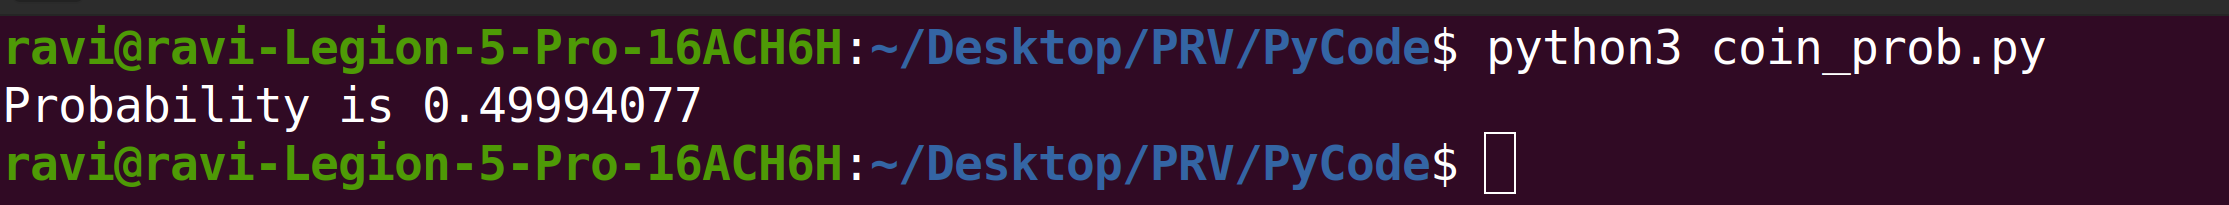
\includegraphics[width=0.75\columnwidth]{../Figures/coin_prob.png}
    \caption{Probability of Getting Heads}
    \label{fig:GettingHeads}
  \end{figure}
\end{frame}

\subsection{Part 2}
\begin{frame}
  \frametitle{Given Condition}
  We define event $A$ as getting 60 \emph{Heads} out of 100 trials (distinct sequence of \emph{Heads} and \emph{Tails}). Given that probability of getting heads is $p$, we have
  \begin{align}
    \Pr(A|p) = p^{60}(1-p)^{40}
    \label{eq:ProbA_p}
  \end{align}

  Using
  \eqref{eq:TotProb},
  \eqref{eq:Dis1}
  in
  \eqref{eq:ProbA_p}
  \begin{align}
    \Pr(A) = \int_{0.4}^{0.6} P(A|p)f(p) dp = \int_{0.4}^{0.6} 5p^{60}(1-p)^{40} dp
    \label{eq:ProbA}
  \end{align}
  
\end{frame}

\begin{frame}
  \frametitle{Using Continuous Bayes Theorem}
  We state the Bayes Theorem for continuous random variables as follows
  \begin{block}{Continuous Bayes Theorem}
    \begin{align}
      f(x|A) = \frac{\Pr(A|x)}{\Pr(A)}f(x)
      \label{eq:ContBayes}
    \end{align}
  \end{block}

  Using
  \eqref{eq:ContBayes},
  \eqref{eq:ProbA_p}
  and
  \eqref{eq:ProbA}
  we have
  \begin{align}
    f(p|A) = \frac{\Pr(A|p) \times f(p)}{\Pr(A)} = \frac{5p^{60}(1-p)^{40}}{\int_{0.4}^{0.6} 5p^{60}(1-p)^{40} dp}
    \label{eq:Dis2}
  \end{align}
\end{frame}

\begin{frame}
  \frametitle{Probability of Heads given event A}
  We are required to find the probability that we get heads on tossing a coin after event A has occured (i.e.) find $\Pr(H|A)$.
  \begin{align}
    \Pr(H|A) = \int_{0.4}^{0.6} \Pr(H|p)f(p|A) dp = \int_{0.4}^{0.6} p\times f(p|A) dp
    \label{eq:FinalHead}
  \end{align}

  Hence
  \begin{align}
    \Pr(H|A) = \frac{\int_{0.4}^{0.6} p^{61}(1-p)^{40} dp}{\int_{0.4}^{0.6} p^{60}(1-p)^{40} dp} = \fbox{0.56}
  \end{align}
    
\end{frame}

\end{document}
